\documentclass[a4paper]{article}
\usepackage[T1]{fontenc}
\usepackage[utf8]{inputenc}
\usepackage{lmodern}
\usepackage[polish]{babel}
\usepackage{makeidx}
\usepackage{amsfonts}
\usepackage{graphicx}


\title{Sieć Neuronowa Rozpoznająca Litery \\ Sprawozdanie}
\author{
Bartłomiej Bułat\\
Konrad Malawski\\
\\
I rok, 2 stopień, Informatyka Stosowana, EAIiE}

\begin{document}

\maketitle

\newpage
\section{Wstęp}

Celem projektu było zaprojektowanie oraz zbadanie właściwości sieci neuronowej mającej za cel rozpoznawanie wielkich liter alfabetu łacińskiego, 
dostępnych jako macierze o rozmiarach 5x7. 

Sieci zaprojektowano przy wykorzystaniu biblioteki Feed-Forward Neural Network for Python - ffnet. Zbudowane sieci uczono zadanych wzorców różnymi 
metodami (Patrz sekcja 2), a następnie sprawdzano ich efektywność w rozpoznawaniu obrazów liter poddawanych coraz to większym zakłóceniom.
2. Wybrane struktury i metody uczenia sieci neuronowych

Podczas przeprowadzanych testów struktura sieci pozoztawała bez zmian. Modyfikowaliśmy jedynie zastosowane algorytmu uczące. Zastosowaliśmy metodę
\verb|mlgraph| generującą standardową wielopoziomową strukturę sieci neuronowej, analogiczną do przedstawionej na Rysunku \ref{rys:graf}.

\begin{figure}[pht]
 \centering
 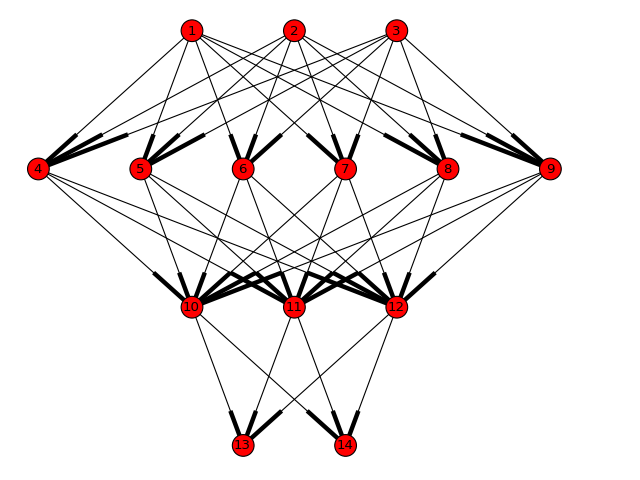
\includegraphics[scale=0.34]{mlgraph}
 \caption{Schemat warstwowej sieci neuronowej}\label{rys:graf}
\end{figure}


Sieć złożona jest z 3 warstw (w tym jednej ukrytej): 
\begin{itemize}
 \item 35 neuronów w warstwie wejściowej - odpowiadojącej ilości elementów macierzy przedstawiającej litery, 
 \item 10 neuronów warstwy ukrytej, 
 \item oraz 26 neuronów warstwy wyjściowej odpowiadające kolejno każdej literze alfabetu.
\end{itemize}

Wybór metod uczenia sieci, celem uzyskania możliwie dużego przeglądu, postanowiliśmy przetestować wszystkie udostępniane przez ,,ffnet'' metody, tj:

\begin{itemize}
 \item \verb|train_momentum| - prostą metodę ze wsteczną propagacją błędów z zachowaniem “momentu”, służącemu zapobieganiu utkwienia sieci w lokalnym minimum (lub siodle),
 \item \verb|train_rprop| - metoda z wsteczną propagacją błędu. Tę samą metodę zastosowano również na zajęciach podczas 2gich zajęć laboratoryjnych,
 \item \verb|train_cg| - metoda gradientu sprzężonego,
 \item \verb|train_bfgs| - metoda opierająca się na algorytmie BFGS,
 \item \verb|train_tnc| - metoda uczenia wielozadaniowego,
\end{itemize}

Na podstawie poniżej umieszczonych wyników testów będzie można ocenić która z metod uczenia sieci najlepiej sprawdziła się w naszym przypadku.

\end{abstract}

\section{Analiza regresji liniowej}
Poniżej przedstawiono przebiegi testów dla każdego z wyżej wspomnianych algorytmów.
Na osi X zaznaczono poziom szumów które dodano do badanych obrazów. Dodawanie szumu wykonano poprzez N-ktorne (gdzie N to “poziom szumu”) wylosowanie punktu w macierzy 5x7 (reprezentującej badaną literę) w którym wykonano odwrócenie wartości logicznej. To znaczy jeżeli dane pole było częścią litery, oznaczaną wartościami“1”, to zmieniano ją na “0”, oraz analogicznie w przeciwnym przypadku.

Przedstawione poniżej wyniki zostały uzyskane przy pomocy wbudowanej funkcji “test” służącej zbadaniu charakterystyk sieci poddawanej testom na podstawie podanego wejścia oraz oczekiwanego wyjścia.

\subsection{Nachylenie}
\begin{figure}[pht]
 \centering
 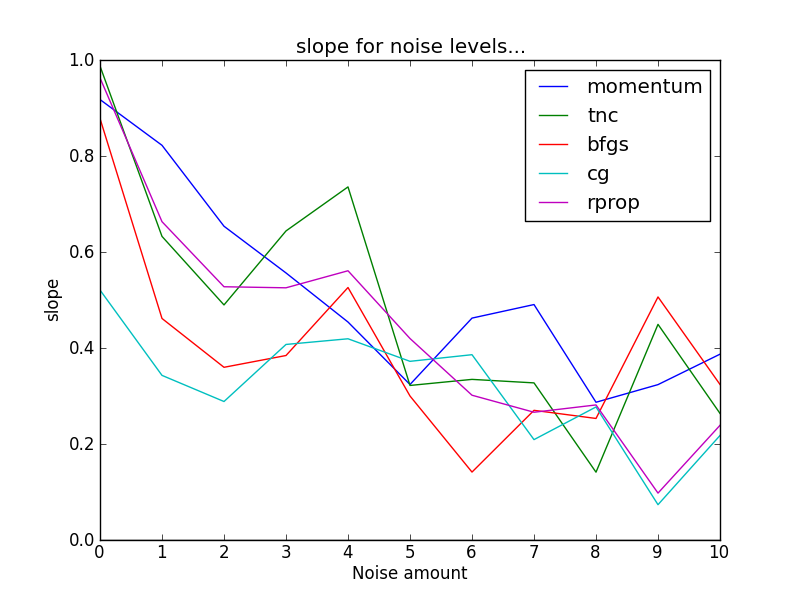
\includegraphics[scale=0.5]{../compare_plots/compare_plot_slope}
 \caption{Wykres wartości slope}\label{rys:plot1}
\end{figure}
Nachylenie (ang. ,,\textit{slope}'') w najlepszym praypadku może przyjąć wartość 1, ponieważ krzywa regresji 
powinna przebiegać pod kątem 45 stopni przez punkt 0,0. Jak widać na Wykresie \ref{rys:plot1},
metody proste bezproblemowo radzą sobie w tym przypadku zanim dodamy zakłucenia do badanych liter.
Metoda gradientu sprzężonego (cg) nie poradziła sobie dbyt dobrze przy zerowym zakłuceniu, jednak warto 
zauważyć iż dodając kolejne zakłucenia wartość nachylenie uzyskana przez tenalgorytm uczenia nie pogarsza się tak drastycznie 
jak w przypadku innych metod.

\subsection{Przesunięcie}
\begin{figure}[pht]
 \centering
 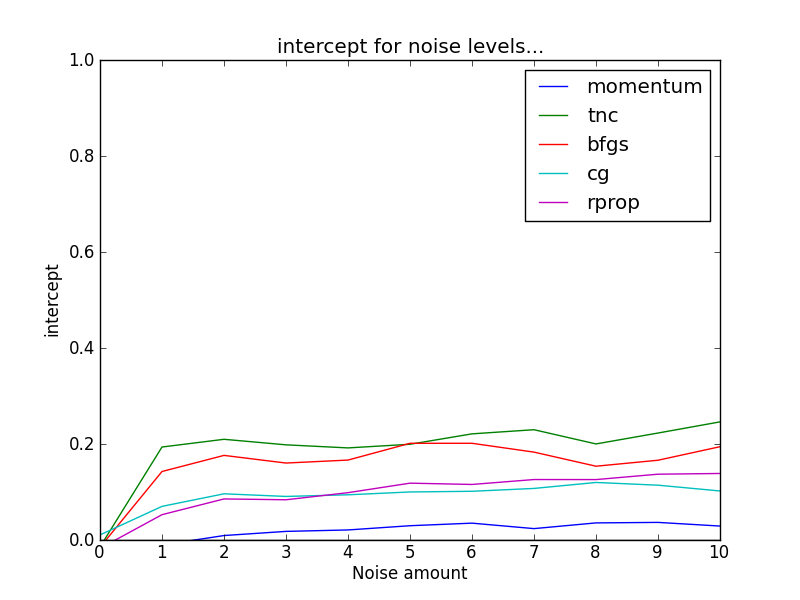
\includegraphics[scale=0.5]{../compare_plots/compare_plot_intercept}
 \caption{Wykres wartości slope}\label{rys:plot1}
\end{figure}
Optymalną wartością przesunięcia (ang. ,,\textit{intercept}'') jest 0. Ponownie widać, że metoda momentum niewiele oddala się od
wartości optymalnej wraz z wzrostem zaszumienia wzorów liter poddawanych próbom rozpoznania.

\subsection{R-Value}
\begin{figure}[pht]
 \centering
 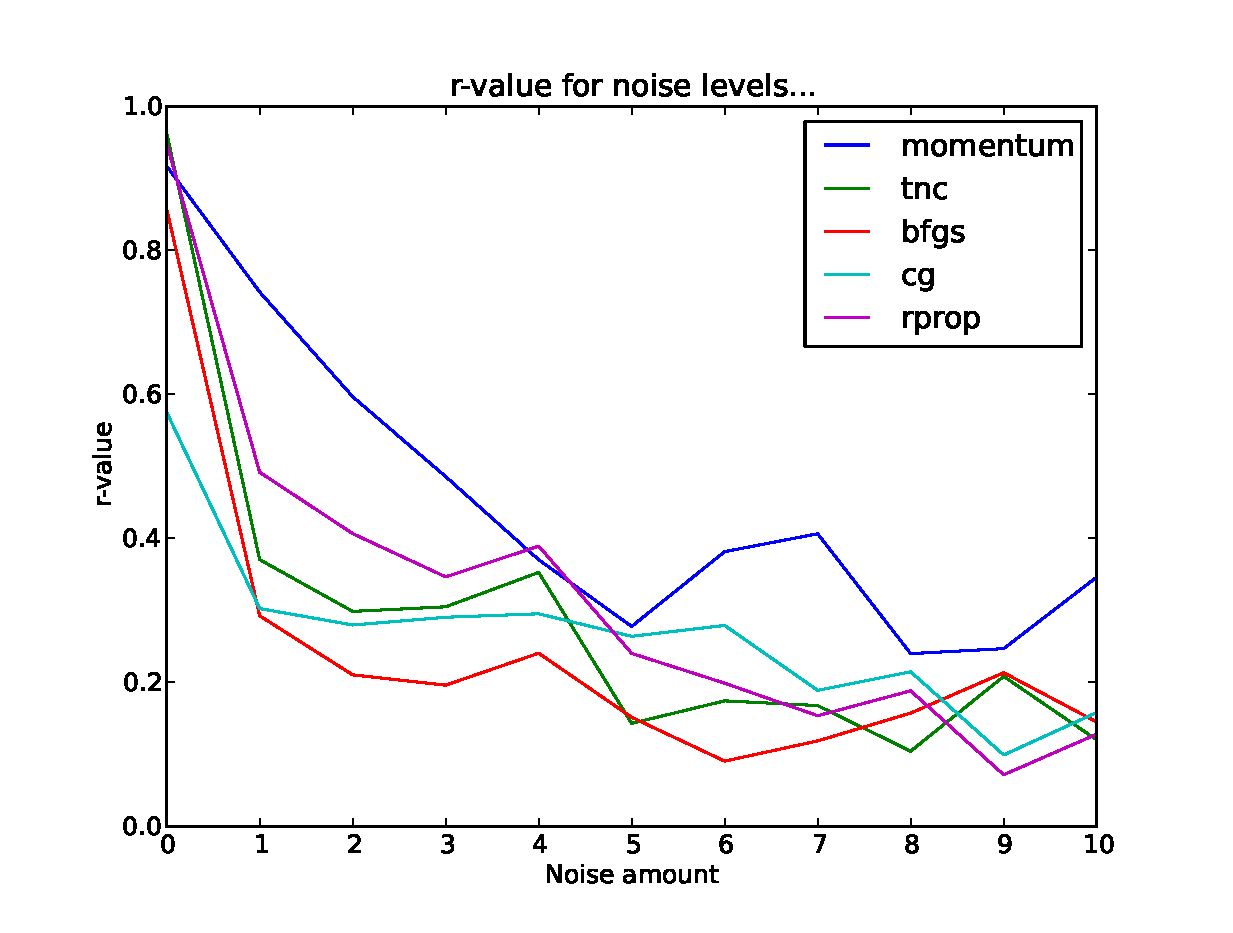
\includegraphics[scale=0.5]{../compare_plots/compare_plot_r_value}
 \caption{Wykres wartości R-Value}\label{rys:plot1}
\end{figure}
r-value jaknajwieksze

\subsection{P-Value}
\begin{figure}[pht]
 \centering
 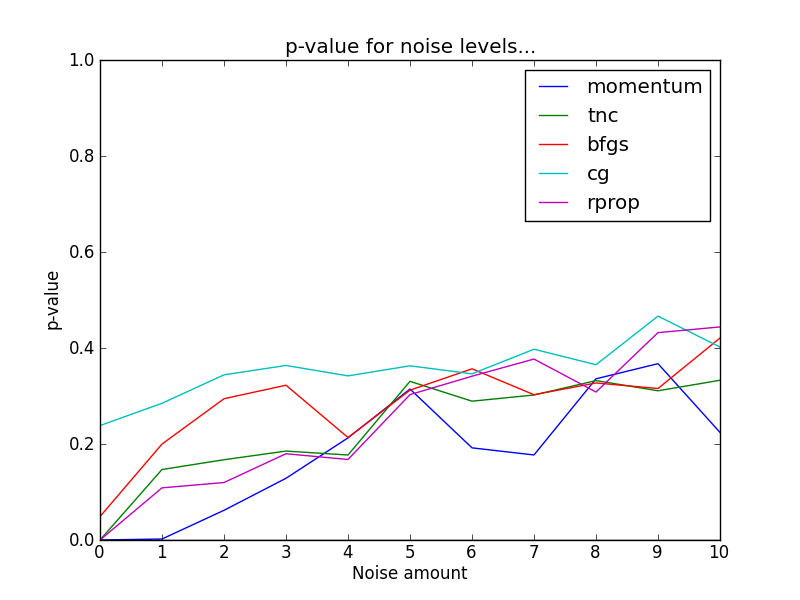
\includegraphics[scale=0.5]{../compare_plots/compare_plot_p_value}
 \caption{Wykres wartości P-Value}\label{rys:plot1}
\end{figure}
p-value jaknajmniejsze

\subsection{Błąd Standardowy - Stderr}
\begin{figure}[pht]
 \centering
 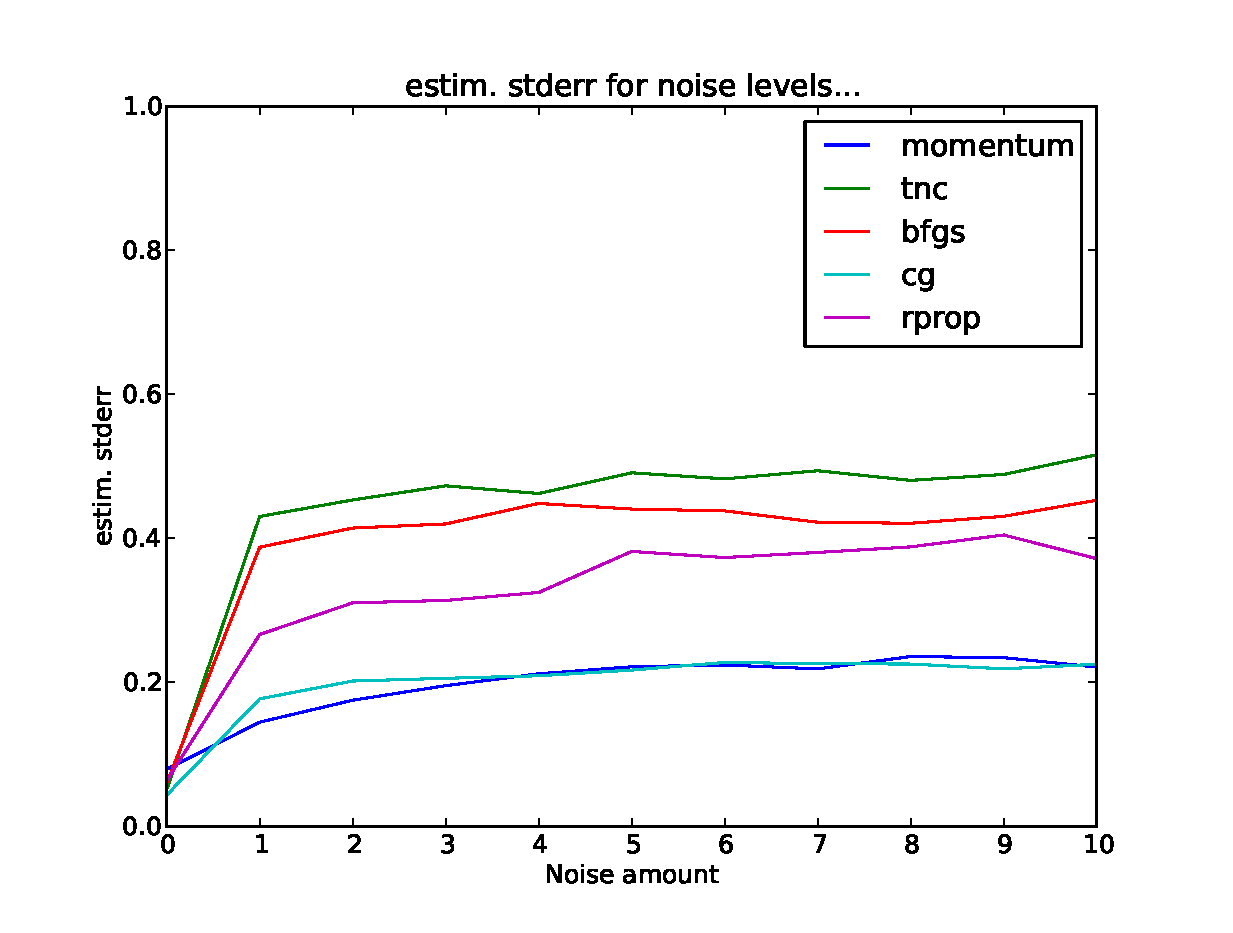
\includegraphics[scale=0.5]{../compare_plots/compare_plot_estim__stderr}
 \caption{Wykres wartości Estimate StdErr}\label{rys:plot1}
\end{figure}
\begin{figure}[pht]
 \centering
 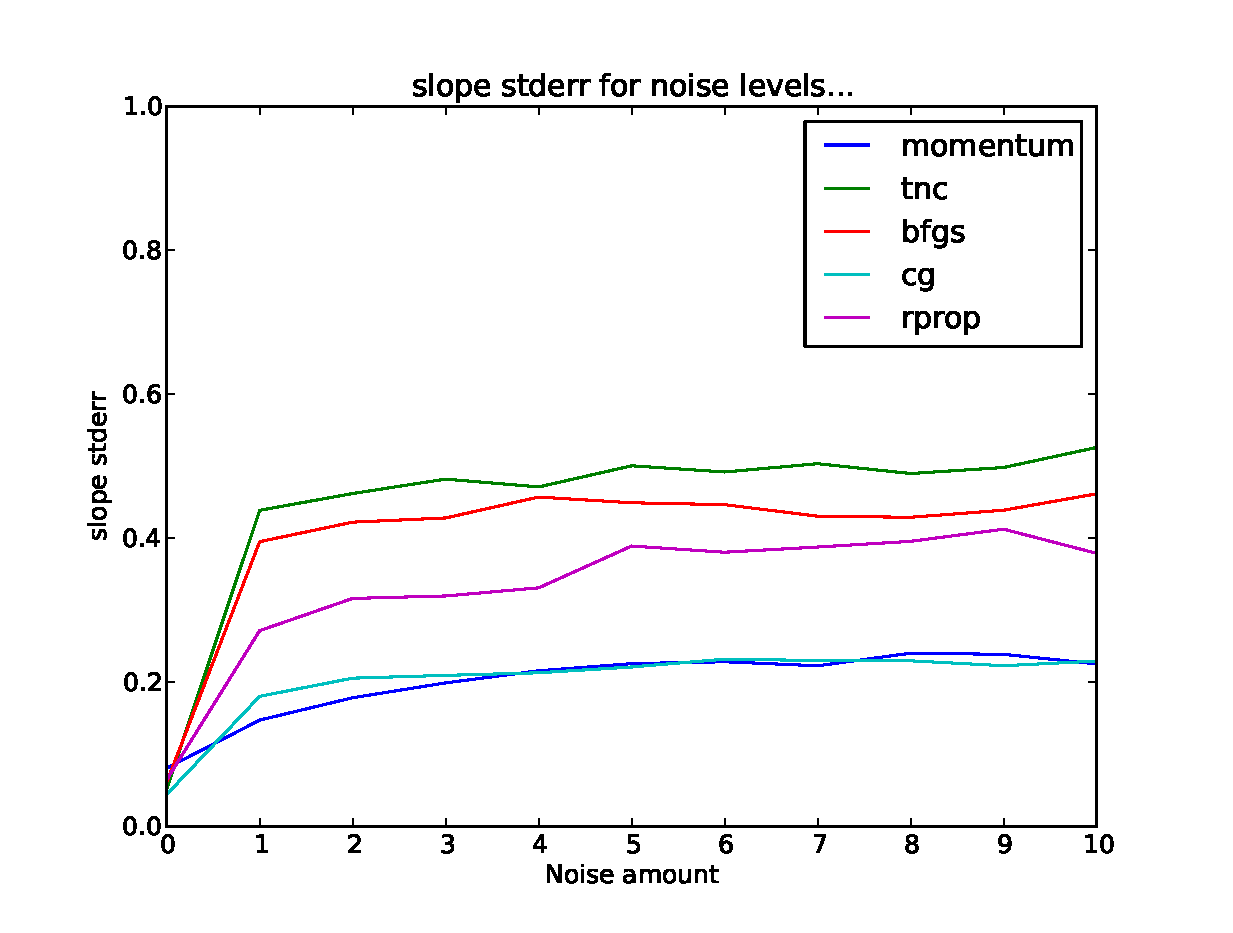
\includegraphics[scale=0.5]{../compare_plots/compare_plot_slope_stderr}
 \caption{Wykres wartości Slope StdErr}\label{rys:plot1}
\end{figure}

Analizując błędy standardowe zastosowanych algorytmów łatwo jest ocenić który z nich
najlepiej ,,nauczył'' naszą sieć. Najgorzej sprawdziła się metoda uczenia wielozadaniowego (wykorzystująca BGFS),
posiadając we wszystkich pomiarach (poza początkowym - z brakiem szumów). Kolejnym algorytmem jest BFGS wspomniany już,
z tym, że tym razem w wersji jedno zadaniowej.

Pozytywnie wyróżniają się bardziej zaawansowane metody, to znaczy: metoda uczenia z gradientem sprzężonym (cg) oraz 
metoda ze wsteczną propagacją błędu z momentum. Wyraźnie widoczna jest różnica w jakości sieci wygenerowanej przy pomocy 
metody ze wsteczną propagacją ,,z'' i ,,bez'' elementu momentum - okazuje się on na tyle dobry iż przyrównuje metodę tą do 
skomplikowanej metody wykorzystującej gradient.

\section{Podsumowanie}
Najlepszą metodą okazała się być metoda uczenia ze wsteczną propagacją błędu z ,,momentem''.
Okazała się nawet skuteczniejsza niż bardziej zaawansowana metoda jaką jest metoda gradientu sprzężonego.

Warto wspomnieć iż przy wszystkich wybranych algorytmach uczących zastosowano domyślne parametry. 
Dalsze testy oraz próby optymalizacji dobranych parametrów mogłyby pozytywnie wpłynąć na uzyskiwaną przez sieci efektywność.

\section{Bibliografia}
\begin{itemize}
 \item Artykuł o analizie regresji liniowej: http://www.mp.pl/artykuly/index.php?aid=10899
 \item Strona domowa projektu ffnet: http://ffnet.sourceforge.net/
\end{itemize}


\end{document}